\section{Comparison to Sockets}\label{sec:comparison-to-sockets}
Since the aim of the API is to replace the existing BSD sockets API, a comparison between both APIs is important.
For this comparison, two implementations of a program which attempts a DNS lookup for a given domain name and connects
to first successful connection attempt, prioritising IPv6 addresses over IPv4 addresses.
To have a fair comparision between the two API, the sockets version must also prioritise IPv6 addresses over IPv4
addresses, since the TAPS version does this internally.
Since a DNS lookup could have a large impact on the total latency, the domain tested is requested multiple times before
running the program under test.
See Appendix~\ref{ch:bsd-sockets-connection-code} for the sockets code and Appendix~\ref{ch:taps-connection-evaluation-code}
for the TAPS code.

\subsection{Latency Comparison}\label{subsec:latency-comparison}
Performance is important for network programming, and as discussed in Chapter~\ref{ch:analysis/requirements} the new
API should have performance similar to BSD sockets (sockets).
A major difference between the two API is how they open connections.
This API does similar things to the sockets version, but does them internally and asynchronously.
For example, the sockets version requires the user to explicitly resolve domain names and race them, whereas TAPS
does this internally.
Since this difference could be significant, a test will be ran to determine which API has the lowest time for opening
connections.
The tests will be executed on a University-provided Linux machine, connected to the University's IPv6 enabled network.
See Appendix~\ref{ch:bash-script-for-latency-testing} for the script used to test the two programs.

\begin{figure}[h]
    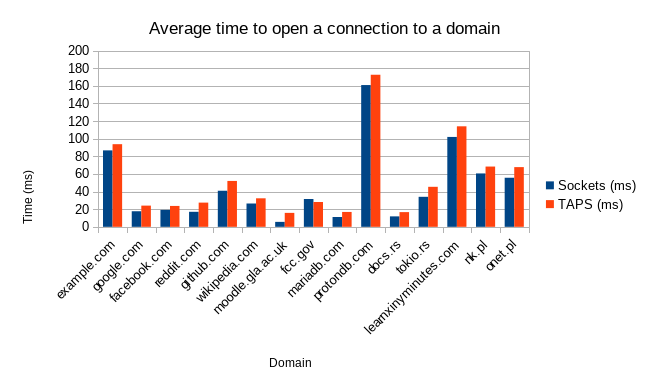
\includegraphics[width=\textwidth]{../data/processed/avg_latency}
    \caption{A graph to show the average time each API takes to connect to a range of domains.}
    \label{fig:latency}
\end{figure}

As shown in Figure~\ref{fig:latency}, TAPS is slightly slower at opening connections in almost every case when compared
to sockets.
This is likely due to TAPS being an asynchronous API.
For the \texttt{Future}'s to be executed, an asynchronous runtime must be created to repeatedly poll each
\texttt{Future}.
Sockets does not have this overhead since it is a synchronous API.
To reduce the impact of this overhead, the programs were modified to open \(10\) connections each time they were ran.

\begin{figure}[h]
    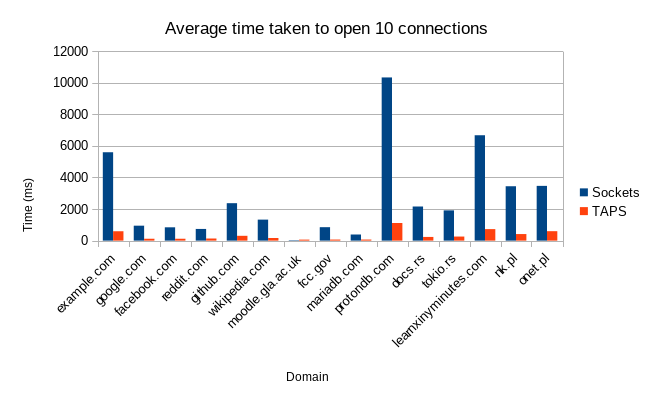
\includegraphics[width=\textwidth]{../data/processed/avg_multi}
    \caption{A graph to show the average time each API takes to open 10 connections to a range of domain.}
    \label{fig:multiLatency}
\end{figure}

Figure~\ref{fig:multiLatency} shows the results of the test after the programs were modified and shows TAPS is takes
less time to open \(10\) connections.
This will be because each connection attempt is executed asynchronously, whereas the sockets version opens each
connection sequentially.

As a result of the two tests, sockets has been shown to have a lower connection-initialisation latency, therefore would
be better suited for short-lived programs, which open a few connections, or programs which would not benefit from an
asynchronous runtime, such as simple single-threaded programs.
An example of this type of program would be cURL\footnote{\url{https://curl.haxx.se}} or
wget\footnote{\url{https://www.gnu.org/software/wget/}}.
Whereas, TAPS would be better suited for programs which open many connections, and can make use of the asynchronous
runtime.
An example would Firefox\footnote{\url{https://www.mozilla.org/en-US/firefox/}} or qBittorrent
\footnote{\url{https://www.qbittorrent.org}}.

%\subsection{Code Comparison}\label{subsec:lines-of-code-comparison}
%While lines of code is not a good metric to determine the quality of code, the substantial difference between the two
%implementations is worth discussing.
%Since sockets is a lower level library than TAPS, more code is required to do the same work as in TAPS .
%Opening a connection with the sockets API requires the following:
%\begin{itemize}
%    \item DNS lookup via \texttt{getaddrinfo}
%    \item Reorder DNS responses to prioritise IPv6 addresses
%    \item Open a socket
%    \item Connect to the remote server
%\end{itemize}
%The TAPS API does this all within \emph{Preconnection}'s \texttt{initiate} method.

%How good is your solution? How well did you solve the general problem, and what evidence do you have to support that?
%
%\section{Guidance}
%\begin{itemize}
%    \item
%        Ask specific questions that address the general problem.
%    \item
%        Answer them with precise evidence (graphs, numbers, statistical
%        analysis, qualitative analysis).
%    \item
%        Be fair and be scientific.
%    \item
%        The key thing is to show that you know how to evaluate your work, not
%        that your work is the most amazing product ever.
%\end{itemize}
%
%\section{Evidence}
%Make sure you present your evidence well. Use appropriate visualisations, reporting techniques and statistical analysis, as appropriate.
%
%If you visualise, follow the basic rules, as illustrated in Figure~\ref{fig:boxplot}:
%\begin{itemize}
%\item Label everything correctly (axis, title, units).
%\item Caption thoroughly.
%\item Reference in text.
%\item \textbf{Include appropriate display of uncertainty (e.g. error bars, Box plot)}
%\item Minimize clutter.
%\end{itemize}
%
%See the file \texttt{guide\_to\_visualising.pdf} for further information and guidance.
%
%\begin{figure}
%    \centering
%    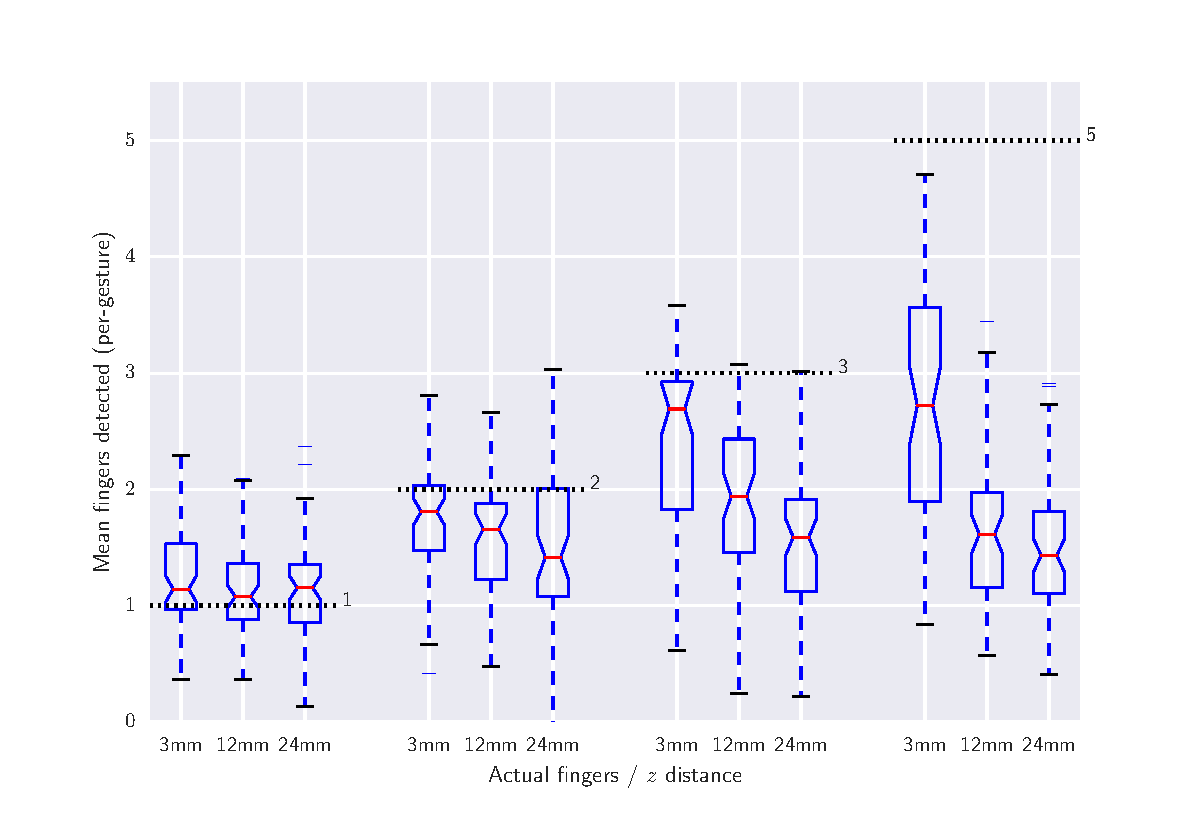
\includegraphics[width=1.0\linewidth]{images/boxplot_finger_distance.pdf}
%
%    \caption{Average number of fingers detected by the touch sensor at different heights above the surface, averaged over all gestures. Dashed lines indicate
%    the true number of fingers present. The Box plots include bootstrapped uncertainty notches for the median. It is clear that the device is biased toward
%    undercounting fingers, particularly at higher $z$ distances.
%    }
%
%    % use the notation fig:name to cross reference a figure
%    \label{fig:boxplot}
%\end{figure}
